\documentclass[a4paper,11pt]{article}


%----------------------------------------------
%	PACKAGE SPECS
%----------------------------------------------
\usepackage[english]{babel}
\usepackage[utf8]{inputenc} % for correct characters
\usepackage[T1]{fontenc}
\usepackage{graphicx} % using pictures
\usepackage[dvipsnames]{xcolor} % colored text
\usepackage{indentfirst}
\usepackage{caption}


%----------------------------------------------
%	ENVIRONMENT SPECS
%----------------------------------------------
\newenvironment{bottompar}{\par\vspace*{\fill}}{\clearpage}

\setlength{\parindent}{2em}
\graphicspath{ {images/} }

\captionsetup[figure]{labelfont={bf},labelformat={default},labelsep=colon,name={Obrázek}}


%----------------------------------------------
%	AUTHOR AND FILE INFO
%----------------------------------------------
\title{Implementace překladače imperativního jazyka IFJ17}
\author{
	Daniel Dolejška (xdolej08)
	\newline
	Petr Ullrich (xullri00)
	\newline
	Lukáš Kulda (xkulda01)
}
\date{prosinec 2017}


%----------------------------------------------
%	CONTENTS
%----------------------------------------------
\begin{document}


%------------------
%	Title page
%------------------
\begin{titlepage}
	\centering
	
	%------------------
	%	Nadpis
	%------------------
	{
		\huge
		\textbf{Implementace překladače imperativního jazyka IFJ17}
	}

	\vspace{1cm}
	
	%------------------
	%	Tým a varianta
	%------------------
	Tým 074, varianta II
	
	\vspace{0.25cm}
	
	%------------------
	%	Aktivní rozšíření
	%------------------
	{
		\large\textbf{Implementovaná rozšíření}
		
		\textsf{UNARY},
		\textsf{BASE},
		\textsf{FUNEXP},
		\textsf{IFTHEN},
		\textsf{BOOLOP}
	}
	
	\vfill
	
	%------------------
	%	Seznam řešitelů s procenty podílu
	%------------------
	\renewcommand{\arraystretch}{1.2}
	\begin{tabular}{ l l r }
		\hline
		Daniel Dolejška	& \textsf{xdolej08}, vedoucí	& 40\% \\ \hline
		Petr Ullrich	& \textsf{xullri00}				& 30\% \\ \hline
		Lukáš Kulda		& \textsf{xkulda01}				& 30\% \\
		\hline
	\end{tabular}

	\vspace{2cm}

	
\includegraphics[width=10cm]{VUT-FIT-logo.pdf}
	
\end{titlepage}


%------------------
%	Page: ToC
%------------------
\newpage

\tableofcontents

\vspace{2cm}
\listoffigures


%------------------
%	Page: 
%------------------
\newpage
\section{Podrobnosti spolupráce} \label{podrobnosti}

\subsection{Rozdělení práce} \label{podrobnosti-rozdeleni}
\noindent
\renewcommand{\arraystretch}{1.2}
\begin{tabular}{ l r l }
	\hline
	Daniel Dolejška	& 40\%	& syntaktický a sémantický analyzátor, testování, dokumentace \\ \hline
	Petr Ullrich	& 30\%	& lexikální analyzátor, dokumentace \\ \hline
	Lukáš Kulda		& 30\%	& generátor, dokumentace \\
	\hline
\end{tabular}

\vspace{4mm}
K nerovnoměrnému rozdělení bodů došlo z důvodu rozdílného rozsahu a náročnosti jednotlivých zpracovávaných modulů.

\subsection{Komunikace a splupráce} \label{podrobnosti-spoluprace}
Komunikace probíhala osobně a pomocí GitLabu, kde měl každý člen týmu vlastní repozitář a mohl tak průběžně ukládat změny a také stahovat změny od ostatních. Každý tak měl možnost vidět kdo, kdy provedl jaké změny.

%------------------
%	Page: 
%------------------
\newpage
\section{Lexikální analýza} \label{lex}
Úlohou lexikálního analyzátoru je rozpoznat jednotlivé vstupní znaky a vytvořit z nich příslušné tokeny.

\subsection{Řešení} \label{lex-reseni}
Hlavní funkcí ovládající lexikální analyzátor je \textbf{Scanner\_GetToken}. Ta cyklicky načítá jednotlivé znaky se standartního vstupu a na základě jejich obsahu mění svůj stav a postupně vytváří token a jeho obsah.

\vspace{2mm}
Cyklus načítání je ukončen v případě, kdy obsah načteného znaku nevyhovuje pravidlům aktuálního stavu automatu. Pokud se automat nachází v konečném stavu nově načtený znak již není součástí aktuálního tokenu a je vrácen tak, aby mohl být načten při dalším volání této funkce, vzniklý token je přes ukazatel v parametru vrácen volající funkci. V případě, kdy se automat v konečném stavu nenachází jedná se o lexikální chybu.

\vspace{2mm}
Po ukončení funkce se vrací číselná hodnota značící zda bylo zpracování úspěšně dokončeno či ne (zastoupena enumerátorem \textsf{ErrorCodes}). Token obsahuje informaci o svém typu a příslušnou hodnotu, která je reprezentována řetězcem znaků a je použita v dalších částech překladače.

\vspace{2mm}
Další implementovanou funkcí je \textbf{Scanner\_UngetToken}, která slouží k vrácení již vytořeného tokenu. Tato funkce předaný token uloží na zásobník tokenů a při dalším volání funkce \textbf{Scaneer\_GetToken} se vrátí již vytvořený token uložený na vrcholu zásobníku, namísto vytváření nového.

\subsection{Konečný automat} \label{lex-fa}
Implementace lexikálního analyzátoru je založena na konečném automatu, který čte jednotlivé vstupní znaky a skládá je do příslušných tokenů. Diagram implementovaného KA je obrázek \ref{fig:automata} na straně \pageref{fig:automata}.

\vspace{2mm}
Dojde-li k lexikální chybě, typ tokenu je nastaven na \textsf{INVALID} a jeho hodnota upřesňuje danou chybu.

\begin{figure}[!htbp]
	\hspace*{-2cm}
	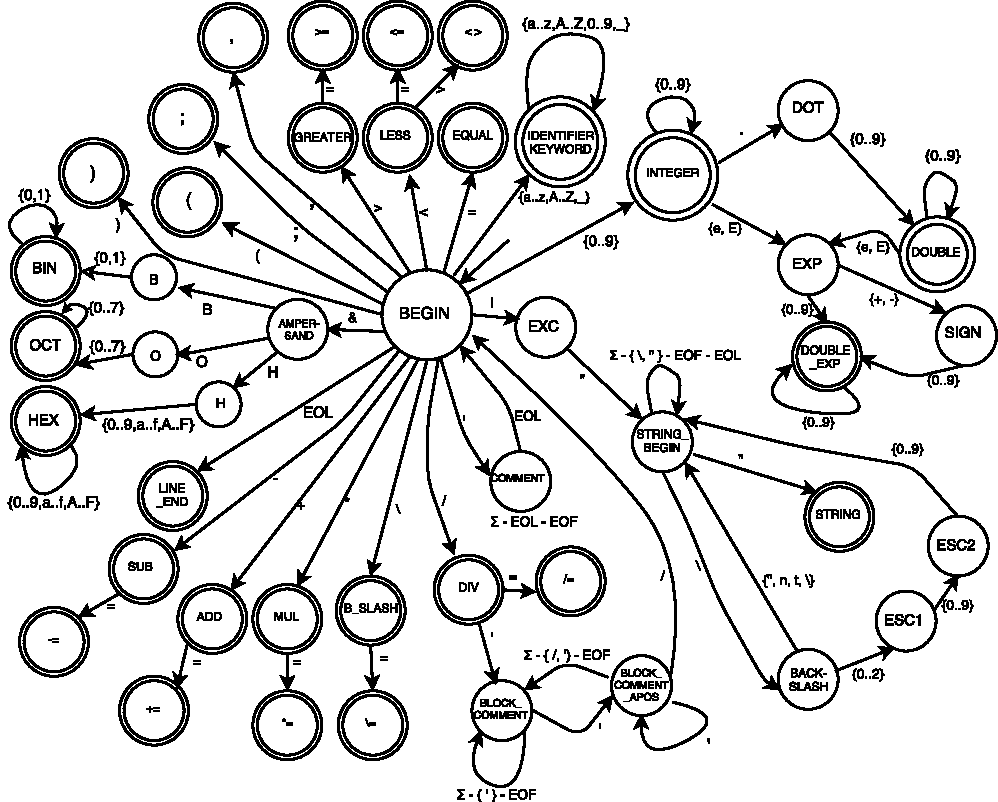
\includegraphics[width=17cm]{ka.pdf}
	\caption{Diagram konečného automatu}
	\label{fig:automata}
\end{figure}


%------------------
%	Page: 
%------------------
\newpage
\section{Syntaktická a sémantická analýza} \label{syse}
Soubor funkcí kontrolující syntaktickou a sémantickou správnost vstupního kódu IFJ17.

\subsection{Princip} \label{syse-princip}
Syntaktický a sémantický analyzátor se skládá z několika funkcí, které odpovídají jednotlivým možným strukturám v jazyce IFJ17. Každá daná funkce načítá tokeny z lexikálního analyzátoru, které následně kontroluje, dále zpracovává a vytváří adekvátní kostru v mezikódu IFJcode17 voláním funkcí generátoru, popřípadě volá další funkce syntaktického a sémantického analyzátoru, které zpracovávají potřebné použité struktury (výrazy, vnořené příkazy apod.).

\subsection{Řešení} \label{syse-reseni}
Syntaktický a sémantický analyzátor se skládá z 19 hlavních funkcí, které slouží ke kontrole syntaktické a sémantické správnosti vstupního kódu a několika dalších pomocných funkcí, které jsou používány pro zjednodušení opakovaných akcí napříč všemi hlavními funkcemi.

\subsubsection{Spuštění překladu} \label{syse-reseni-uvod}
Zpracování začíná v hlavní funkci \textbf{Parser\_ParseInitial}, která vytvoří výchozí úvodní instrukce výstupního programu a dále cyklicky zpracovává příchozí tokeny. Tato úvodní funkce pracuje na stejném principu jako funkce pro zpracování vnořeného kódu, přijímá pouze značně omezený seznam typů tokenů: \textit{deklarace funkce}, \textit{definice funkce}, \textit{definice scope}. 

\vspace{2mm}
Po přijetí očekávaných klíčových slov volá odpovídající funkce, které načítají další tokeny, kontrolují jejich správnost a dále je zpracovávají. Při přijetí tokenu neočekávaného typu analyzuje chybu a vrací odpovídající chybový kód hlavní funkci celého programu.

\subsubsection{Vnořený kód} \label{syse-reseni-vnoreny_kod}
Funkce pro zpracování obecného vnořeného kódu (\textbf{Parser\_ParseNestedCode}) slouží jako křižovatka, která na základě prvního příchozího tokenu volá odpovídající funkci pro zpracování očekávané struktury.

\vspace{2mm}
Dále také rozhoduje, zda je vůbec možné v dané situaci danou strukturu použít – tato rozhodnutí dělá především na základě seznamu zanoření, který určuje, v jaké struktuře se aktuálně vnořený kód zpracovává (zda se jedná o větev podmínky, cyklus či funkci).

\vspace{2mm}
V případě, že tato funkce obdrží token, který by mohl mít speciální význam – klíčové slovo, které nebylo očekáváno a pro vnořený kód nemá žádný smysl (ovšem může se jednat o ukončení nadřazené struktury – konec definice funkce, cyklu apod.), vrací se o úroveň výše, a funkci, která jej zavolala, tento token předává. Ta rozhodne o jeho správnosti.

\subsubsection{Zpracování funkcí} \label{syse-reseni-funkce}
O zpracování funkcí v programu se starají 3 funkce, kde každá z nich má konkrétní účel – jedna funkce pro deklaraci funkce (\textbf{Parser\_ParseFunctionDeclaration}), jedna pro její definici (\textbf{Parser\_ParseFunctionDefinition}) a jedna zpracovává volání těchto funkcí (\textbf{Parser\_ParseFunctionCall}).

\vspace{2mm}
Funkce pro deklaraci a definici funkcí jsou volány z hlavní úvodní funkce syntaktického a sémantického analyzátoru. Funkce pro volání funkcí jsou volány z funkcí pro zpracování výrazů.

\subsubsection{Zpracování podmínek} \label{syse-reseni-podminky}
Podmínky zpracovávají dvě funkce – první \textbf{(Parser\_ParseCondition}), která zpracovává prvotní podmínku a \textsf{ELSE} bez další následující podmínky, a druhá (\textbf{Parser\_ParseSubCondition}), která zpracovává další libovolný počet navazujících \textsf{ELSEIF} podmínek.

\vspace{2mm}
Druhá funkce pro zpracování navazujících \textsf{ELSEIF} podmínek zpracovává pouze tyto typy – v případě, že obdrží token značící kompletní ukončení podmínky či začátek \textsf{ELSE} větve, vrací se postupně na nejvyšší úroveň, dokud se nevrátí do první funkce, která daný token zpracuje sama.

\vspace{2mm}
Tyto funkce dále využívají funkci pro zpracování výrazů (k vyhodnocení pravdivostní hodnoty v podmínce) a funkci pro zpracování vnořeného kódu.

\subsubsection{Zpracování cyklů} \label{syse-reseni-cykly}
Funkce pro zpracování cyklu \textsf{DO WHILE} (\textbf{Parser\_ParseLoop\_Do}) funguje principiálně stejně jako všechny ostatní hlavní funkce. Využívá funkcí pro zpracování pravdivostních výrazů a funkci pro zpracování vnořeného kódu pro zpracování instrukcí v cyklu.

\vspace{2mm}
Cyklus je složen z dvou návěstí, počátečního a konečného. Po počátečním návěstí následují instrukce pro vyhodnocení výrazu a podmíněný skok na konečné návěstí v případě nesplnění podmínky.

\subsubsection{Zpracování výrazů} \label{syse-reseni-vyrazy}
Pro zpracování funkcí slouží dvě funkce, první funkce (\textbf{Parser\_ParseExpression}) ke zpracování hlavního výrazu a druhá funkce (\textbf{Parser\_ParseSubExpression}) která zpracovává podvýrazy v závorkách.

\begin{figure*}
	\centering
	\renewcommand{\arraystretch}{1.3}
	\begin{tabular}{ l r }
		OPERÁTOR					& PRIORITA 	\\ \hline\hline
		*, /						& 1			\\ \hline
		\textbackslash				& 2			\\ \hline
		+, -						& 3			\\ \hline
		<, <=, <>, >, >=, =			& 4			\\ \hline
		\textsc{NOT}				& 5			\\ \hline
		\textsc{AND}, \textsc{OR}	& 6			\\ \hline
	\end{tabular}
	
	\caption{Precedenční tabulka operátorů}
	\label{fig:precedence_table}
\end{figure*}

Tyto funkce využívají funkce pro převod příchozích tokenů na postfixový výraz. Po jednom dané tokeny funkcím odesílají a ty je zpracovávají a vytvářejí z nich postfixový výraz. Po přijetí tokenu neočekávaného typu (například neočekávané klíčové slovo nebo, \textsf{EOL}) je výraz ukončen a vyhodnocen.

\vspace{2mm}
Po ukončení postfixového výrazu jsou volány funkce na převod tohoto výrazu na instrukce, ty na základě informací v položkách postfixového seznamu vytvoří seznam instrukcí pro zpracování výrazu.

\vspace{2mm}
Tento převod probíhá ve dvou částech – první zpracování vzniklého postfixového řetězce vytvoří odpovídající seznam instrukcí na základě příchozích proměnných a operací. Druhé zpracování validuje správnost datových typů v operacích ve vzniklé posloupnosti instrukcí a v případě nutnosti provést implicitní převod datových typů, vloží mezi ostatní instrukce potřebnou instrukci pro požadovaný převod datových typů.
Výsledné instrukce jsou pak ze speciálního seznamu překopírovány do hlavního seznamu instrukcí.

\subsection{Pomocné datové struktury} \label{syse-struktury}
Syntaktický a sémantický analyzátor využívá několik pomocných datových struktur pro jednodušší předávání informací mezi funkcemi. Mezi ně patří zásobník, seznam či tabulka s rozptýlenými položkami.

\subsubsection{Zásobník} \label{syse-struktury-zasobnik}
Zásobník je v hojném použití při převodu příchozích tokenů na postfixový výraz. Dále je také využíván při zpracování volání funkcí ve výrazech, k uložení tokenů popisujících parametry dané funkce či při „vracení“ tokenů lexikálnímu analyzátoru.

\subsubsection{Seznam} \label{syse-struktury-seznam}
V tomto projektu jsou využity jednosměrně i dvousměrně vázané seznamy. Mezi zástupce jednosměrně vázaného seznamu patří postfixový seznam, ve kterém je uložen zpracovaný postfixový výraz, seznam tokenů či seznam zanoření, který je používán především funkcí pro zpracování vnořeného kódu.

\subsubsection{Tabulka s rozptýlenými položkami} \label{syse-struktury-tabulka}
Tato struktura byla použita při implementaci tabulky symbolů překladače na základě dané varianty zadání.


%------------------
%	Page: 
%------------------
\newpage
\section{Generátor} \label{gen}
Vytváří, ukládá a dále pracuje s instrukcemi mezikódu IFJcode17.

\subsection{Řešení} \label{gen-reseni}
Pomocí implementovaných funkcí pro skládání řetězců vytvoří instrukci jako jeden řetězec z názvu instrukce a případně jednoho či více symbolů obsahujících informace o jednotlivých argumentech, který následně uloží jako poslední prvek do dvousměrně vázaného seznamu. Tyto funkce sice umožňují snazší složení řetězců, ale vytváří tak alokované textové řetězce, které je potřeba následně uvolnit.

\vspace{2mm}
Každá instrukce mezikódu má svou vlastní funkci, která přijímá pouze argumenty, které daná instrukce vyžaduje. Při výpisu tiskne jednotlivé instrukce na standartní výstup, každou na nový řádek tak, jak jsou v seznamu uloženy.

\subsection{Pomocné datové struktury} \label{gen-struktury}
Tento modul využívá dvousměrně vázaný seznam pro ukládání vytvořených instrukcí a jejich následný výpis.

	
\end{document}